\chapter{Исследовательская часть}

Целью данного исследования является анализ производительности различных алгоритмов нахождения расстояний Левенштейна и Дамерау-Левенштейна на различных строках, в зависимости от их длины и характера. В ходе исследования измерялось время выполнения программ на различных реализациях (итеративная, рекурсивная, рекурсивная с мемоизацией и алгоритм Дамерау-Левенштейна).


Технические характеристики используемого микроконтроллера STM32F767ZIT6 \cite{lit3}:
\begin{itemize}
	\item 32 бит, 
	\item 216 МГц, 
	\item ARM Cortex-M7, 
	\item Flash 2 Мбайт, 
	\item RAM 512 Кбайт;
\end{itemize}

Для исследования использовались строки разной длины (от 3 до 9 (включительно) символов). Алгоритмы выполнялись на микроконтроллере с использованием MicroPython.

\section {Результаты исследования}

Была построена зависимость времени выполнения алгоритмов от длины строк (таблица с результатами замеров представлена под номером \ref{tab:performance} сравнительный график представлен на рисунке \ref{tab:performance}).

\begin{table}[H]
    \centering
    \small
    \begin{tabular}{@{}rccccc@{}}
        \toprule
        Длина слов & Рекурсивный Л.(с) & Рекурс. + кэш Л.(с) & Итеративный Л.(с) & Итерат. Д.-Л. (с) \\ \midrule
        1          & 0.00099945   & 0.00099945 & 0.00300550             & 0.00099683      \\
        2          & 0.00299788   & 0.00602508 & 0.00598407             & 0.00600028      \\
        3          & 0.01799178   & 0.01100206 & 0.00499701             & 0.00600147      \\
        4          & 0.08699870   & 0.01299977 & 0.00800014             & 0.01199961      \\
        5          & 0.45722175   & 0.01900077 & 0.01100016             & 0.01510143      \\
        6          & 2.61085057    & 0.02775168 & 0.01549363             & 0.01852417      \\
        7          & 12.134186980   & 0.03571510 & 0.02200031             & 0.02300000      \\
        8          & 73.384949920   & 0.05216599 & 0.02795100             & 0.03400254      \\
        9          & 375.0456602600  & 0.05351448 & 0.03253579             & 0.03846931      \\ \bottomrule
    \end{tabular}
    \caption{Время выполнения для различных алгоритмов и длин слов}
    \label{tab:performance}
\end{table}

\begin{figure}[H]
    \raggedright    
    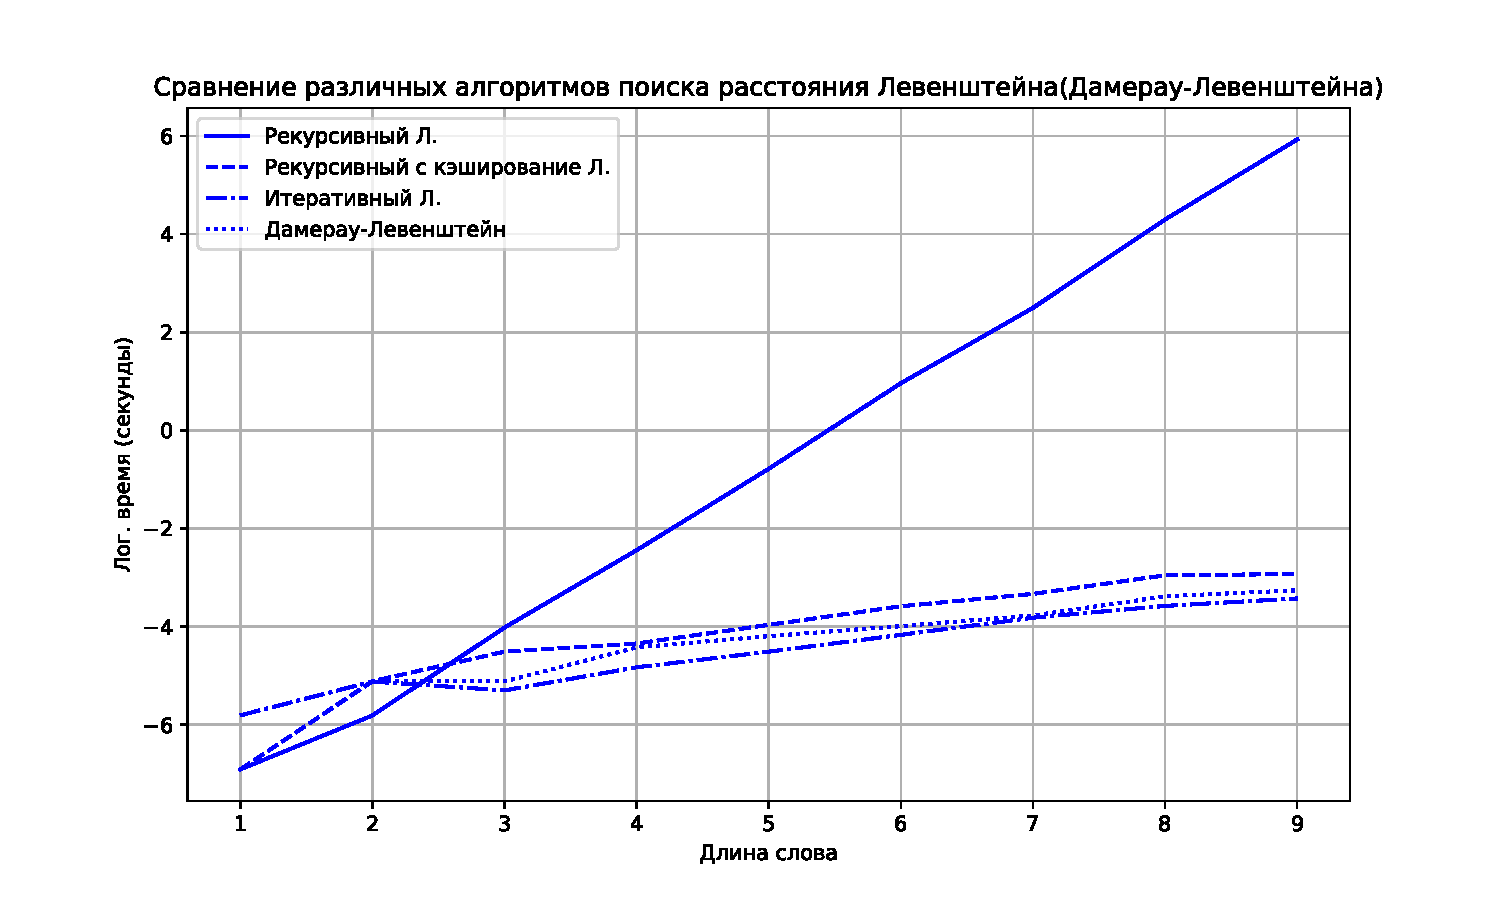
\includegraphics[width=180mm]{images/graph_comparation}
    \caption{Сравнительный график зависимости времени выполнения алгоритмов от длины строк}
    \label{images:graph_comparation}
\end{figure}



\section*{Вывод}

В ходе исследования была проанализирована производительность различных алгоритмов нахождения расстояний Левенштейна и Дамерау-Левенштейна. Итеративные алгоритмы показали лучшее время выполнения по сравнению с рекурсивными. Использование мемоизации улучшило производительность рекурсивного метода, но он все равно оказался менее эффективным по сравнению с итеративным подходом.
